\section{MPI}

\begin{frame}{History}
    \begin{columns}
    
        \begin{column}{0.55\textwidth}

    \begin{itemize}
        \item \textbf{Before 1990's}: Many libraries. 

        Writing code was a \alert{\textbf{difficult}} task.

        \vspace{0.2cm}
        \hrule{}
        \vspace{0.2cm}
        {\textbf{Models commonly adopted: Message Passing Model}}
        
        An application \alert{\textbf{passes messages}} among processes in order to perform a task.

        e.g. Job assignment, Results of sub-problems...
        
    \end{itemize}
    \end{column}

        \begin{column}{0.45\textwidth}
            \begin{itemize}
                \item Supercomputing '92

                Defined a \alert{\textbf{standard interface}}

                \item 1994

                MPI-1

                \item 2025.6.5
            
                MPI-5.0 Standard Release
            \end{itemize}
        \end{column}
    \end{columns}
    %\footnotetext{https://mpitutorial.com/tutorials/mpi-introduction/}

    %\footnotetext{https://www.mpi-forum.org/docs/}
\end{frame}

\begin{frame}{What is MPI}
    MPI, a \alert{\textbf{M}}essage \alert{\textbf{P}}assaing \alert{\textbf{I}}nterface.

    There exists many implementations:
    \begin{itemize}
        \item OpenMPI
        \item Intel-MPI
        \item MPICH
        \item HMPI (Hyper-MPI)
        \item ......
    \end{itemize}

    \textbf{Kindly Reminder}: Please do not mess up MPI implementations with MPI standard.
\end{frame}


\begin{frame}{Installation}
    \begin{itemize}
        \item OpenMPI
        
            Lab0
        \item Intel-MPI: Included in \href{https://www.intel.cn/content/www/cn/zh/developer/tools/oneapi/toolkits.html}{Intel- neAPI}
        
            Can be installed using spack

        \item HMPI: \href{https://support.huawei.com/enterprise/zh/doc/EDOC1100228708/c5d7ef16}{Huawei}
    \end{itemize}
\end{frame}

\begin{frame}[fragile]{Hello MPI World!}
    \begin{minted}[fontsize=\scriptsize]{c}
#include <mpi.h>
#include <stdio.h>
int main(int argc, char** argv) {
    MPI_Init(&argc, &argv);
    int world_size;
    MPI_Comm_size(MPI_COMM_WORLD, &world_size);
    int world_rank;
    MPI_Comm_rank(MPI_COMM_WORLD, &world_rank);
    char processor_name[MPI_MAX_PROCESSOR_NAME];
    int name_len;
    MPI_Get_processor_name(processor_name, &name_len);
    printf("Hello world from processor %s, rank %d out of %d processors\n",
    processor_name, world_rank, world_size);
    MPI_Finalize();
    return 0;
}
    \end{minted}
\end{frame}

\subsection{Basic Concepts}

\begin{frame}{Communicator}
    \begin{block}{Definition}
        A communicator defines a group of processes that have the ability to communicate with one another.
        
        Each process has a \alert{\textbf{unique rank}}.
    \end{block}
\end{frame}


\begin{frame}{Communicator (cont.)}
\begin{columns}
    \begin{column}{.6\textwidth}
        \begin{itemize}
        \item MPI\_COMM\_WORLD
        \end{itemize}
        \begin{figure}
            \centering
            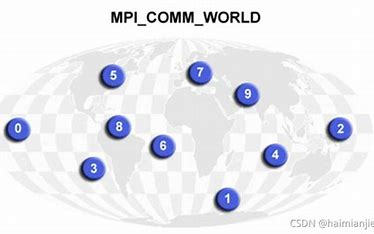
\includegraphics[width=\linewidth]{day8_am/img/mpi/mpi_comm_world.png}
            \caption{}
            \label{fig:mpi_comm_world}
        \end{figure}
    \end{column}
\end{columns}

\end{frame}


\begin{frame}{Communicator (cont.)}
\begin{columns}
    \begin{column}{.6\textwidth}
    \begin{itemize}
        \item MPI\_COMM\_SPLIT

        \begin{itemize}
            \item comm: The communicator that will be used as the basis for the new communicators.
            \item color: Which new communicator each processes will belong.
            \item key: The ordering (rank) within each new communicator.
            \item new\_comm: [OUT]
        \end{itemize}
    \end{itemize}
    \end{column}
        \begin{column}{.4\textwidth}
        \begin{figure}
            \centering
            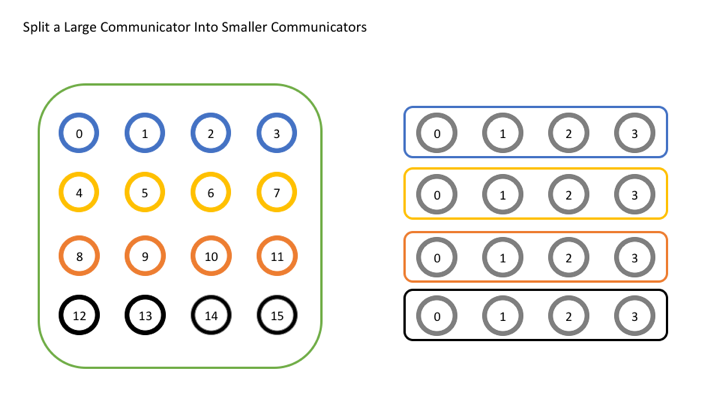
\includegraphics[width=1.0\linewidth]{day8_am/img/mpi/commsplit.png}
        \end{figure}
    \end{column}
\end{columns}

\end{frame}

\begin{frame}{Blocking vs Non-blocking}
    \begin{columns}
        \begin{column}{.5\textwidth}
            \textbf{\large Blocking}

            It does not return until the message data and envelope have been \alert{\textbf{safely stored away}} so that the sender is free to modify the send buffer. 
            
            The message might be copied directly into the \alert{\textbf{matching receive buffer}}, or it might be copied into a \alert{\textbf{temporary system buffer}}.
        \end{column}
        \begin{column}{.5\textwidth}
            \textbf{\large Non-blocking}

            A nonblocking call initiates the operation, but does not complete it. 
            
            They will return \alert{\textbf{almost immediately}}.
            
        \end{column}
    \end{columns}
\end{frame}

\begin{frame}{Order}
    \textbf{\large Messages are non-overtaking}
    
    Order is preserved.(Only under single thread)

If a sender sends two messages in succession to the same destination, and both match the same receive, then this operation cannot receive the second message if the first one is still pending. 

If a receiver posts two receives in succession, and both match the same message, then the second receive operation cannot be satisfied by this message, if the first one is still pending.
\end{frame}

\begin{frame}{Fairness}
    MPI makes \alert{\textbf{no guarantee}} of fairness in the handling of communication.

    There may be starvation.

    \begin{example}
        Rank1 $\rightarrow ^{send}$ Rank0

        Rank2 $\rightarrow^{send}$ Rank0

        Rank0 $\leftarrow^{receive}$ from any source.
    \end{example}
\end{frame}